% Ventilated cavities on a flexible surface-piercing hydrofoil
%
% Every number in this manuscript is produced by the repository it documents.
% The figures are written by docs/paper/make_figures.py; the tabulated scalars
% come from verify_vent.py, whose output docs/VENTILATION.md also tabulates.
% No experimental data have been digitised: the values attributed to Harwood,
% Young & Ceccio (2016) are the ones stated in the text of that paper.
%
% Build:  pdflatex ventilation && bibtex ventilation && pdflatex ventilation
%
\documentclass[11pt,a4paper]{article}

\usepackage[T1]{fontenc}
\usepackage[utf8]{inputenc}
\usepackage{lmodern}
\usepackage[british]{babel}
\usepackage{amsmath,amssymb}
\usepackage{graphicx}
\usepackage[margin=25mm]{geometry}
\usepackage[font=small,labelfont=bf]{caption}
\usepackage{booktabs}
\usepackage{natbib}
\usepackage{siunitx}
\usepackage[colorlinks=true,allcolors=blue]{hyperref}

\bibpunct{(}{)}{;}{a}{}{,}
\graphicspath{{figures/}}
\sisetup{detect-all,per-mode=power}

\newcommand{\Fnh}{\mathit{Fn}_h}
\newcommand{\ARh}{\mathit{AR}_h}
\newcommand{\We}{\mathit{We}}
\newcommand{\dd}{\mathrm{d}}

\title{\bf Ventilated cavities on a flexible surface-piercing hydrofoil}

% The author list is to be completed by the corresponding author.
\author{%
  I.\,M.\ Viola\thanks{Corresponding author: \texttt{i.m.viola@ed.ac.uk}}\\[2pt]
  \small School of Engineering, Institute for Energy Systems,\\
  \small University of Edinburgh, Edinburgh, EH9 3FB, UK}

\date{}

\begin{document}
\maketitle

\begin{abstract}
\noindent
Atmospheric ventilation limits the load a surface-piercing hydrofoil can carry:
air entrained into separated suction-side flow forms a gas cavity that removes
most of the suction, and the wetted and ventilated states coexist. Predictive
models are sectional relations closed by a lifting line: they resolve neither the
chordwise pressure nor the cavity thickness, and hold the hydrofoil rigid. The present paper asks whether it
can instead be predicted inside a partitioned fluid--structure solver at a
fidelity that keeps the coupling well posed. To this end a free-wake
source--doublet panel method is extended by an exact linearised free surface, a
negative image obtained by mesh doubling with the source strengths sign-flipped
on the image half; by a cavity whose pressure, length and thickness are solved as
a mixed doublet--source boundary-value problem; and by a hysteretic regime
machine that advances only on commit. The
free-surface condition holds to \num{1.7e-16} of the doublet scale, and the image
antisymmetry, solved for rather than imposed, to \num{2.4e-14}. Ventilation
removes \SI{44}{\percent} of the lift and moves the
centre of pressure from $0.34c$ to $0.19c$, against the $3c/16$ of a
supercavitating section. The computed mean cavity closure angle lies within
\SI{4}{\percent} of the value measured at washout, and bi-stability spans
ten degrees of incidence. Softening the strut deepens its suction margin by a
third and moves the operating point across the boundary beyond which a
ventilated cavity is sustained, so a lifting surface's load limit can now be
assessed together with its structural response.
\end{abstract}

\section{Introduction}
\label{sec:Intro}

Surface-piercing hydrofoils carry the loads of sailing craft, of surface-effect
ships and of tidal-turbine support structures, and their load limit is set not by
stall but by ventilation. Air drawn from the free surface into separated flow on
the suction side forms a gas cavity at, or close to, atmospheric pressure; the
suction that the cavity replaces is lost, and with it up to
\SI{70}{\percent} of the lift~\citep{Breslin1959}. The phenomenon has been
studied since the first surface-piercing propellers~\citep{Wetzel1957}, and the
governing similarity groups are the immersed aspect ratio $\ARh = h/c$, the
depth-based Froude number $\Fnh = u/\sqrt{gh}$ and the Weber number, with the
incidence $\alpha$ setting whether separated flow exists at
all~\citep{Harwood2016}.

Three features make ventilation hard to predict. The first is that the cavity
pressure is fixed by the atmosphere while the reference pressure varies with
depth, so the cavitation number is stratified and the cavity is long at the
waterline and short at the tip. The second is that the flow regimes are
bi-stable: fully wetted, partially ventilated and fully ventilated flows coexist
over overlapping regions of the parameter space, and which one is realised
depends on the history~\citep{Harwood2016}. The third is that formation and
elimination are controlled by different mechanisms - formation by the connection
of separated flow to the free surface, elimination by the re-entrant jet at
cavity closure - so a single threshold cannot describe both.

The state of the art in prediction is sectional. The classical linearised cavity
solutions of \citet{Acosta1955} for a partial cavity and of \citet{Tulin1953} for
a supercavity give the cavity length as a function of the single parameter
$\Psi = \sigma_c/(2\alpha_{2\mathrm{D}})$, and the cavity lift slope follows from
the same hodograph construction. In \citet{Harwood2016} these are fitted by
smooth rational relations, closed spanwise by an elliptic loading and rescaled to
three dimensions by Helmbold's small-aspect-ratio formula, and the stability of a
fully ventilated cavity is decided by the mean angle $\bar{\Phi}$ of its closure
line from the horizontal, with $\bar{\Phi} > \ang{45}$ giving an upstream
re-entrant jet. That model reproduces the measured regime boundaries and the
scale of the lift loss, and it is the reference against which any richer model
must be judged.

What a sectional model cannot supply is what a structural designer needs. It
gives no chordwise pressure distribution, so it cannot be integrated to a load on
a deforming surface. It prescribes the cavity as a pressure condition with no
thickness, so the cavity's displacement effect on the circulation is absent. Its
closure angle is a measured input rather than a computed output. Its regime is
selected by hand from the branch the analyst expects. It is steady, so it carries
no added mass and no wake memory. Above all it is one-way: the hydrofoil is
rigid, so the twist that a real strut develops under load - which changes the
incidence and therefore the quantity that decides inception - cannot enter.
Ventilation of a flexible surface-piercing hydrofoil has consequently been
studied experimentally~\citep{Harwood2020} but not, to the authors' knowledge,
predicted by a coupled model in which the regime itself responds to the
deformation.

The present paper aims to address the following research question: can
atmospheric ventilation - its inception, its effect on the loads, and its
elimination - be predicted within a partitioned fluid--structure solver at a
fidelity sufficient to keep the coupling well posed, and does the resulting model
reproduce the published sectional relations and measured scalars of
\citet{Harwood2016} while supplying the three-dimensional and two-way
information that those relations cannot?

The approach is to add three things to a verified partitioned solver and to test
each against a reference of the same standing. A free surface is added as an
exact negative image, so that the linearised high-Froude condition holds to
round-off and can be verified as an identity rather than as an agreement. A
cavity boundary-value problem is added in which the doublet strength is
prescribed on cavity panels by the dynamic condition and the source strength is
solved, so that the cavity acquires a thickness and the computed pressure on the
cavity is a result rather than an imposition. A regime machine is added that
advances only on commit, which is what keeps the coupled load a function of the
displacement and therefore keeps quasi-Newton acceleration applicable. The
Methodology (\S\ref{sec:Method}) states the formulation and the conventions that
pin its signs; the Results (\S\ref{sec:Results}) verify the parts that can be
verified exactly, compare the parts that can be compared with a stated
percentage, and report the parts for which no reference of equal standing exists,
in that order, closing with what the model supplies beyond the sectional one; the
Conclusions (\S\ref{sec:Conclusions}) return to the research question and state
the limitations that bound the answer.

\section{Methodology}
\label{sec:Method}

\subsection{The three fields and their coupling}
\label{subsec:Fields}

The fluid is an unsteady source--doublet panel method with a free wake, in the
Morino formulation, carried unmodified from a separate verified
implementation~\citep{Viola2026a}. The body is closed and thick, the doublet
strength $\mu$ is the unknown on wetted panels, the source strength is
$\sigma = -\mathbf{n}\cdot\mathbf{u}_{\mathrm{rel}}$, and the pressure follows
from the surface gradient of $\mu$ through the unsteady Bernoulli equation with
the $\partial\phi/\partial t$ term evaluated from the doublet history. The
structure is a three-dimensional finite-element solid with trilinear
incompatible-mode hexahedra, a generalised-$\alpha$ integrator, and Newton loops
on the residual formed from $\int B^{\mathsf{T}}\boldsymbol{\sigma}$ rather than
from $Ku$, so that a nonlinear constitutive law is a change of one class. The
coupling is partitioned: loads are lumped from panel centroids to the wetted
finite-element surface by a partition of unity that reproduces the collocation
point, so force, moment and virtual work transfer exactly, and the interface is
built once on the reference configuration so that the coupling residual is a
fixed function of the displacement.

Five states carry the computation, and only one is new. The panel state, the
structural model, the committed structural level and the interface transfer are
those of the underlying solver. The fifth is the ventilation state, which holds
the parameters, the mirror maps and - advancing only when a time level is
committed - the regime, the per-station cavity length, the cavity depth and the
mean closure angle. Everything a coupling subiteration computes lives in a
transient dictionary and is discarded. That separation is not tidiness: a
strongly coupled step re-solves the same time level several times, and a regime
that flipped inside the subiteration would stop the load being a function of the
displacement, because the regimes are bi-stable.

\subsection{The free surface as an exact negative image}
\label{subsec:Image}

At high Froude number the free-surface condition linearises to $\phi = 0$ on the
undisturbed plane, which is satisfied identically by a flow field antisymmetric
about that plane. The condition is imposed here by geometry rather than by a
constraint. The strut of immersion $h$ is meshed together with its mirror above
the waterline, giving a single closed body of span $2h$ with a full-chord section
on the plane and both far tips pinched, and the source strengths on the image
half are overridden as
%
\begin{equation}
  \sigma_{\mathrm{image}} = -\sigma_{\mathrm{real}}\!\circ\!P ,
  \label{eq:imagesigma}
\end{equation}
%
where $P$ is the panel permutation induced by the reflection. The doublet
antisymmetry is \emph{not} imposed: it emerges from the solve, and that it does
is the test that the image is correct.

Figure~\ref{fig:mesh} shows the doubled mesh and the potential it produces on the
plane. Three properties fall out of the construction rather than being
engineered. The builder is bit-exactly mirror-symmetric, because the section
ordinates are even in the spanwise coordinate and an odd number of stations
places a node row on the plane, so the symmetry residual is exactly zero rather
than small. The yaw rotation is about the spanwise axis and preserves the
symmetry bit-exactly. The trailing-edge weld and the tip pinch of the geometry
update act per station and commute with the reflection, so the symmetry survives
every geometry update of a coupled march.

One hazard has to be stated beside the construction, because it is a plausible
wrong turn that fails silently. Mirroring leaves
$-\mathbf{n}\cdot\mathbf{u}_{\mathrm{rel}}$ unchanged for an onset with no
spanwise component, so on a doubled mesh the unflipped solve is bit-for-bit the
rigid-wall answer. A bare call to the underlying solver on a ventilating state
therefore returns the zero-Froude solution, quietly, with about twice the lift.
For the same reason the lift coefficient of the doubled state is a near
cancellation and not the answer: resultants are taken over the immersed half on
the reference area $s_{\mathrm{ref}} = hc$.

\begin{figure}[t]
  \centering
  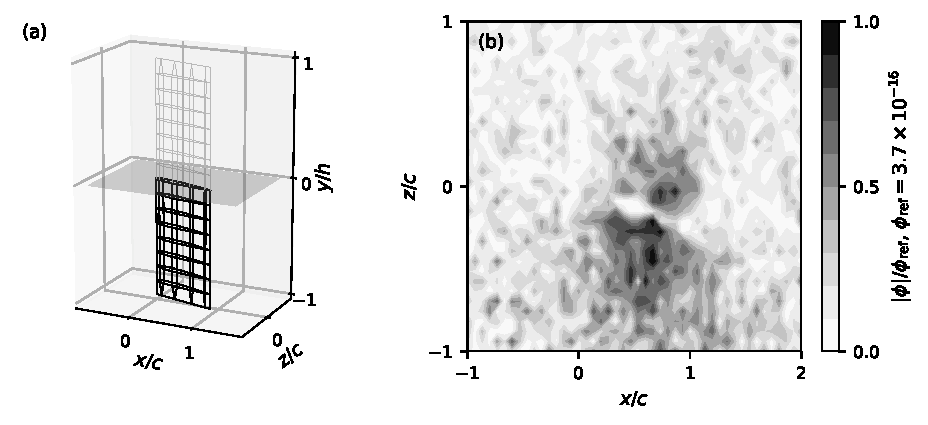
\includegraphics[width=\textwidth]{mesh}
  \caption{The doubled surface-piercing strut and the potential it produces on
    the free-surface plane, at $\alpha = \ang{14}$, $\Fnh = 2.5$,
    $\ARh = 1$: (a) the immersed half in black, its image in grey and the plane
    shaded, with the span drawn vertically because the span is the depth;
    (b) the magnitude of the perturbation potential on the plane, normalised by
    the largest doublet strength, at a level that is round-off and carries no
    structure.}
  \label{fig:mesh}
\end{figure}

The image wake, however, cannot be convected. With $\phi$ antisymmetric the
perturbation velocity obeys $\mathbf{v}'(R\mathbf{x}) = -R\,\mathbf{v}'(\mathbf{x})$
while the onset obeys $\mathbf{v}(R\mathbf{x}) = +R\,\mathbf{v}(\mathbf{x})$, so a
mirror-consistent advection would require the perturbation to vanish. Left to
convect, the image wake drifts off the mirror position, the influence matrix
stops commuting with the permutation, and the free-surface condition is lost
progressively over a march. The image wake is therefore projected onto the
mirror-symmetric set after every shedding step, with the real half
authoritative. The discarded drift has a physical reading: on the plane the
chordwise and vertical perturbations are antisymmetric and vanish, while the
depthwise one is symmetric and does not, so the projected-out drift is the
linearised wave elevation rate. It is reported as a diagnostic, and it is the
quantitative measure of how far below the model's valid Froude range a run has
been pushed.

\subsection{The cavity boundary-value problem}
\label{subsec:Cavity}

The reference pressure is the local still-water pressure
$P_{\mathrm{atm}} + \rho g z'$, with $z'$ the depth below the undisturbed
surface. Against that reference a wetted panel carries the dynamic pressure
alone - which is what the underlying solver already computes - and a ventilated
panel carries $C_p = -\sigma_c(z')$ with
%
\begin{equation}
  \sigma_c(z') = \frac{P_{\mathrm{atm}} + \rho g z' - P_c}{\tfrac12\rho u^2}
               = \Delta\sigma + \frac{z'}{h}\,\frac{2}{\Fnh^{2}} ,
  \label{eq:sigmac}
\end{equation}
%
where $\Delta\sigma = (P_{\mathrm{atm}} - P_c)/(\tfrac12\rho u^2)$ vanishes for
natural atmospheric ventilation and is positive for a vaporous or pressurised
cavity, which the same code covers. Two consequences follow. A hydrostatic
reference term must be \emph{rejected} rather than merely left unset when
ventilating, since it would double-count the still-water field. And the
still-water part of the pressure integrates to the buoyancy of the immersed
volume and is deliberately absent from the fluid load, as are weight and gravity
on the structure: both are body forces for a caller to apply, so a static
deflection compared with an experiment is missing both.

On a cavity panel the dynamic condition fixes the pressure, hence the total
surface speed $q_c = u\sqrt{1+\sigma_c}$, hence the doublet strength by
chordwise integration from the detachment point,
%
\begin{equation}
  \frac{\partial\mu}{\partial s} = V_s
    - \mathbf{u}_{\mathrm{rel}}\!\cdot\!\hat{\mathbf{s}} ,
  \qquad
  V_s = \pm\sqrt{q_c^{2} - V_v^{2}} ,
  \label{eq:dynamic}
\end{equation}
%
with the spanwise component $V_v$ lagged one iteration and $\mu$ continuous with
the wetted solution at detachment. The unknown on a cavity panel is then the
source strength, which is the cavity's transpiration, and linearised the
thickness is
%
\begin{equation}
  t(s) = \frac{1}{V_s}\int_{s_{\mathrm{d}}}^{s}
         \bigl[\sigma - \sigma_{\mathrm{wetted}}\bigr]\,\dd s' ,
  \qquad t(s_{\mathrm{d}}) = 0 .
  \label{eq:thickness}
\end{equation}
%
The per-panel choice of unknown is a mask over the assembled system, so the
cavity costs one extra solve per iteration and no new kernel. Because $\mu$ is
prescribed on the cavity, the surface-velocity and pressure evaluations return
the cavity pressure by construction; that the computed $C_p$ on cavity panels
equals $-\sigma_c(z')$ to the surface-gradient discretisation error is therefore
an end-to-end test of the whole cavity path rather than a tautology.

Three decisions inside the cavity iteration are load-bearing. The cavity is
parameterised by a continuous per-station length with a fractional weight on the
closure panel, never by a boolean mask: a boolean mask makes the load
piecewise-constant in the displacement, the cavity chatters between adjacent
panels, and quasi-Newton acceleration fits its least-squares system to a
staircase. The cavity extent is read off the baseline wetted pressure and
never off the pressure the cavity has itself imposed, because the dynamic
condition makes the latter equal the cavity pressure on the cavity, so the
margin would be identically zero there and the cavity would collapse at every
iteration. And the iteration is cold-started from the committed extent every
time, so that the converged extent does not depend on the subiteration path.

\subsection{Inception, regimes and elimination}
\label{subsec:Regimes}

A panel method has no boundary layer, so separation is an assumption and is made
visible as one: the stall angle and the pressure-recovery fraction are inputs,
they live in the state where they can be inspected, and every case reports them
as inputs. Inception requires three things together - a connected region of
ventilation-ready flow covering more than a stated fraction of the immersed
suction area, a path from that region to the free surface, and a broken surface
seal - and the seal is taken to break at the stall angle or when air is injected.
The air path is seeded on separation at the waterline station rather than
on pressure, because with a negative image the loading and hence $C_p$ go to zero
at the free surface while $\sigma_c(0) = 0$ for natural ventilation, so a
pressure-seeded flood fill reads $0 < 0$ exactly where the air must enter and may
never start.

The regime follows \citet{Harwood2016}: with $D$ the cavity depth,
$D = 0$ is fully wetted, $D = h$ with $\bar{\Phi} < \ang{45}$ is fully
ventilated, and anything else is partially ventilated. The closure angle is
measured from the horizontal, $\Phi = \arctan|\dd z'/\dd x_{\mathrm{closure}}|$,
and the convention is pinned by its limiting case: a cavity of uniform length has
$\dd x_{\mathrm{closure}}/\dd z' = 0$, hence $\Phi = \ang{90}$ and a jet directed
straight upstream, which is the classical two-dimensional re-entrant jet and the
canonical unstable case. Spanwise taper is what stabilises a ventilated cavity,
by sweeping the jet sideways. Persistence asks only whether ventilation-ready
flow remains, never again whether the seal is broken, and that asymmetry between
formation and persistence is the hysteresis: it is structural, not a
threshold with a dead band. Elimination is decided by the same closure-angle
criterion, and its scaling is compared with the semi-theoretical washout boundary
%
\begin{equation}
  \Fnh = \frac{\pi}{4}
   \sqrt{\frac{\tfrac{\pi}{2}\ARh^{4} - 4\ARh^{3} + 18\ARh^{2} + 8\ARh}
              {2.31\,C_L\,(\pi \ARh^{3} - 2\pi \ARh^{2} + 3\pi \ARh + 4)}} ,
  \label{eq:washout}
\end{equation}
%
which \citet{Harwood2016} derive from the elliptic loading, the unity-slope
closure condition and the long-cavity relation.

Finally, the cavity front advances at a finite speed, limited to a stated number
of chords of cavity per chord of travel, and the limit bounds the cavity that the
\emph{load} sees rather than only the next step's starting point. Without it the
extent reaches its equilibrium in one step, the load is a step function of time,
and the structural response measures the time step rather than the flow.

\subsection{Cases and base values}
\label{subsec:Cases}

The model depends on the flow only through $\alpha$, $\Fnh$, $\ARh$, the Weber
number and $\Delta\sigma$, and on the structure through the ratio of elastic to
dynamic pressure. Results are reported nondimensionally. The dimensional base
values that convert them back are a chord $c = \SI{1}{\metre}$, an immersion
$h = \SI{1}{\metre}$, a speed $u = \SI{1}{\metre\per\second}$ and a density
$\rho = \SI{1000}{\kilogram\per\cubic\metre}$, so the dynamic pressure is \SI{500}{\pascal};
$\Fnh$ is imposed directly rather than through $g$, so each case stands for any
combination of speed, immersion and gravity with the same $\Fnh$. The structural
material is isotropic with Poisson's ratio $0.3$ and density
\SI{1200}{\kilogram\per\cubic\metre}, and Young's modulus is stated per case. Meshes carry $8$
to $16$ chordwise panels per surface and $6$ to $16$ spanwise strips per
immersed half, doubled by the image; the solid is lofted on the immersed half so
that its outer surface is the wetted surface, and is clamped at the immersed tip.

\section{Results}
\label{sec:Results}

\subsection{The sectional relations are reproduced, and their limits measured}
\label{subsec:Sectional}

Figure~\ref{fig:sectional} compares the implemented sectional model with the
closed forms it is built from. The two analytic limits of the cavity lift slope
are recovered to machine precision, $a_0(0) = 6.283185307180$ against
$2\pi$ and $a_0(\infty) = 1.570796326795$ against $\pi/2$, which is the test that
catches a plausible misreading of the constant in the denominator of that
relation. Against Acosta's partial cavity the rational fit is within
\SI{1.1}{\percent} in $\Psi$ over $0.2 \le L \le 0.4$ and \SI{4.0}{\percent} at
$L = 0.5$, while in $L$ the same fit is \SI{8.7}{\percent} low at $L = 0.5$ and
\SI{33.5}{\percent} low at $L = 0.05$. The comparison that means anything is the
one in $\Psi$, because $\dd\Psi/\dd L$ is large near the branch join; a test
written on $L$ reads as the failure of a fit that is correct. On the supercavity
branch the fit is within \SI{5}{\percent} of Tulin's solution over
$1.25 \le L \le 2.6$ and degrades to $-\SI{40}{\percent}$ at $L = 9.2$ and
$-\SI{63}{\percent}$ at $L = 23.3$, where the simplified long-cavity relation is
the better one. That simplified relation is not an approximation to Tulin's:
Tulin's length grows as $\sigma^{-2}$ and it as $\sigma^{-1}$, so their ratio
diverges and the interval over which they agree is inherited by everything the
washout boundary says.

Two properties of the fits are recorded because they look like defects and are
not. The lift slope is not monotone: it peaks at $7.2022$ at $L = 0.511$, above
$2\pi$, and undershoots its own limit by \SI{0.93}{\percent} near $L = 10$ before
approaching $\pi/2$ from below. And the length fit saturates at $100.54$ as
$\Psi \to 0$ rather than diverging, because its denominator has no positive real
root. The blend used here across the hodograph singularity that both classical
solutions share is monotone in $\Psi$, the largest increment along increasing
$\Psi$ being $-\num{4.3e-4}$.

\begin{figure}[t]
  \centering
  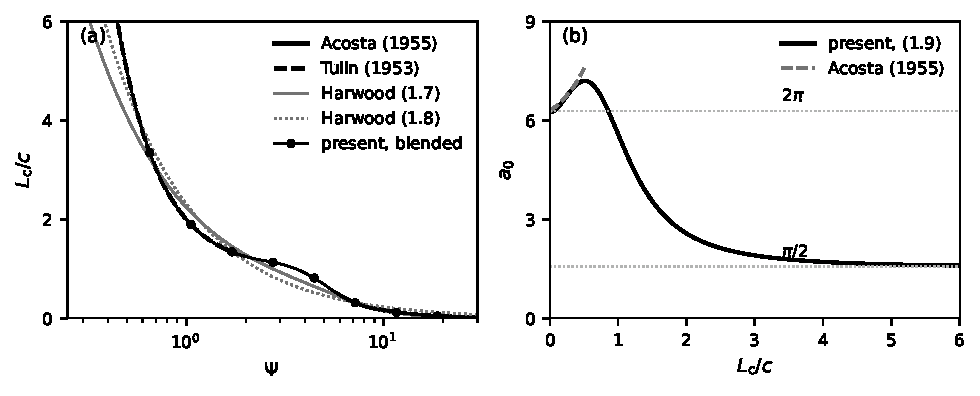
\includegraphics[width=\textwidth]{sectional}
  \caption{The sectional cavity model against the closed forms it is built from:
    (a) cavity length versus the cavity parameter, with Acosta's partial cavity,
    Tulin's supercavity, the two rational fits and the blend used here;
    (b) the cavity lift slope versus cavity length, with Acosta's slope and the
    two analytic limits.}
  \label{fig:sectional}
\end{figure}

\subsection{The free surface is exact, and the transfer conservative}
\label{subsec:Exactness}

Table~\ref{tab:exact} lists the quantities that are identities of the
construction rather than agreements between models, measured at
$\alpha = \ang{14}$, $\Fnh = 2.5$ on $160$ immersed panels. The mesh symmetry
residual is exactly zero. The image doublet strength cancels the mirror of the
real one to \num{2.4e-14} although it is solved for and not imposed, and the
image wake strength to \num{2.7e-14}. The potential on the free-surface plane is
\num{1.7e-16} of the largest doublet strength, and figure~\ref{fig:mesh}b shows
that what remains carries no spatial structure. Flipping the sign in \eqref{eq:imagesigma} reproduces
the underlying rigid-wall solve bit-for-bit, which converts the hazard of
\S\ref{subsec:Image} from a warning into an asserted property. Force, moment and
virtual work pass through the load lumping and the interface transfer at
\num{1.5e-16} or below, and the pressure floor never lowers a pressure, the
largest reduction being exactly zero - a cavity raises the suction-side pressure,
which is why lift is lost, and asserting the sign on pressures rather than on
forces avoids folding in the sign of the normal.

\begin{table}[t]
  \centering
  \caption{Quantities verified at round-off, at $\alpha = \ang{14}$,
    $\Fnh = 2.5$, $\ARh = 1$, on $160$ immersed panels. The first six are the
    free surface; the last four are the load path.}
  \label{tab:exact}
  \small
  \begin{tabular}{lc}
    \toprule
    quantity & error \\
    \midrule
    mirror symmetry of the doubled strut            & \num{0.0e+00} \\
    image doublet strength plus mirror of the real one & \num{2.36e-14} \\
    image source strength plus mirror of the real one  & \num{6.63e-15} \\
    image wake strength plus mirror of the real one    & \num{2.73e-14} \\
    potential on the free-surface plane, relative      & \num{1.70e-16} \\
    unflipped image minus the underlying solve         & \num{0.0e+00} \\
    total force through the load lumping               & \num{1.51e-16} \\
    total force through the interface transfer         & \num{1.13e-16} \\
    total moment through the load lumping              & \num{9.29e-17} \\
    virtual work across the interface                  & \num{0.0e+00} \\
    largest pressure the cavity lowered                & \num{0.0e+00} \\
    \bottomrule
  \end{tabular}
\end{table}

The near cancellation warned of above is quantified here: the immersed-half lift
coefficient is $0.17428$ on $s_{\mathrm{ref}} = hc$, while the whole doubled mesh
returns $0.00407$. The doubled value is not exactly zero because the pressure is
quadratic in a velocity whose tangential part does not simply mirror; scaling it
by two to recover a plausible lift would be a real error wearing a plausible
face.

\subsection{The wetted surface-piercing baseline}
\label{subsec:Wetted}

Figure~\ref{fig:depth} contrasts the free surface with a rigid wall, which is the
comparison that a sign error passes every other test. The negative image drives
the sectional loading towards zero at the waterline, the shallowest strip
carrying $0.434$ of the peak, while the positive image places the maximum
on the plane, the shallowest strip carrying $1.000$ of the peak and the
peak itself being $1.98$ times the free-surface one. A sign error therefore
roughly doubles the lift while leaving every other diagnostic intact.

Refinement separates two statements that are easy to conflate. The circulation of
the shallowest strip falls as $\Delta y^{0.74}$, from $0.549$ to $0.118$ of its
maximum as the immersed half is refined from four to thirty-two strips, so the
loading vanishes at the waterline in the limit as the exact condition requires.
The strip's pressure-integrated sectional force, in contrast, converges to
$0.42$ of the peak and does not vanish: with an even station count no panel
straddles the plane, and the strip retains a non-circulatory contribution from
the large depthwise perturbation velocity there. The exact statement is the one
carried by the potential in table~\ref{tab:exact}; the panel loading vanishes
only in the limit.

\begin{figure}[t]
  \centering
  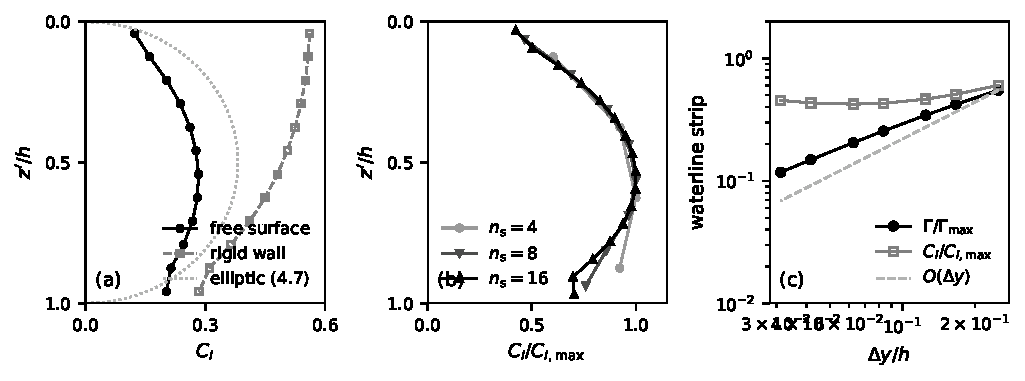
\includegraphics[width=\textwidth]{depth_loading}
  \caption{Sectional loading against depth for the wetted strut at
    $\alpha = \ang{10}$, $\Fnh = 2.5$, $\ARh = 1$: (a) the free-surface image
    against a rigid-wall image and the elliptic shape; (b) the normalised shape
    at three spanwise resolutions; (c) the waterline strip's circulation and
    sectional force against the strip width.}
  \label{fig:depth}
\end{figure}

The measured lift slope of the wetted strut is $C_L/\sin\alpha = 1.3453$, which
is $0.900$ of Helmbold's value at $\ARh = 1$ and $0.506$ of the value at
$2\ARh$. The effective aspect ratio of a surface-piercing strut is the immersed
one, because the negative image makes the waterline behave as a tip; using
$2\ARh$ is the rigid-wall image and moves the lift slope by tens of per cent
while looking plausible. The panel method and the Helmbold-corrected sectional
model are different models, so the \SI{10}{\percent} difference is reported to
the per cent and not verified.

\subsection{The cavity: planform, thickness and pressure}
\label{subsec:CavityResults}

Figure~\ref{fig:planform} shows the solved cavity at $\alpha = \ang{16}$,
$\Fnh = 2.0$. The cavity is longest at the waterline and shortest at the tip,
reaching the trailing edge at the surface and $0.09c$ at the deepest station,
because the cavitation number is stratified by \eqref{eq:sigmac}. Both sectional
reference models give the same shape and a longer cavity near the surface, the
lifting line reaching $35.5c$ and the Helmbold chain $7.6c$ where the panel method
saturates at the trailing edge; near the waterline the sectional length is
formally indeterminate, since $\sigma_c$ and the sectional incidence vanish
together, and the panel method's saturation is what it can legitimately say.

The thickness of \eqref{eq:thickness} vanishes at detachment and grows aft, reaching $0.15c$ at the
shallowest of the three stations plotted, and the cavity encloses a volume of
\num{4.3e-2} chords cubed over the immersed half. That thickness is a qualitative
output and is reported rather than verified, for two measured reasons. A third of
the cavity panels carry a slightly negative thickness, the smallest being
$-0.012c$, which a linearised transpiration integral does not forbid but a cavity
does. And the closure residual, the thickness that remains at the point where the
cavity is required to close, reaches $0.87$ of the local scale rather than
vanishing, which is why the pressure rule and not the thickness rule sets the
extent by default. The thickness is therefore used here to show that the cavity
has a displacement effect at all - which a prescribed-pressure sectional cavity
does not - and not as a predicted cavity shape.

\begin{figure}[t]
  \centering
  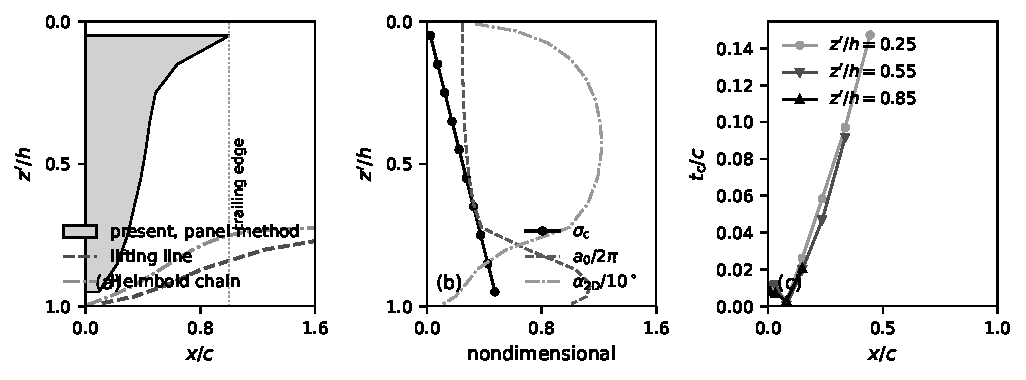
\includegraphics[width=\textwidth]{cavity_planform}
  \caption{The solved cavity at $\alpha = \ang{16}$, $\Fnh = 2.0$, $\ARh = 1$:
    (a) the cavity planform against the two sectional reference models;
    (b) the cavitation number, the cavity lift slope and the sectional incidence
    against depth; (c) the solved cavity thickness at three depths.}
  \label{fig:planform}
\end{figure}

Figure~\ref{fig:pressure} is the end-to-end test of the cavity path, that is
of \eqref{eq:dynamic} together with the mixed solve and the pressure evaluation. At each of
three depths the wetted suction peak of $-3.05$ is replaced by a plateau at the
local $-\sigma_c(z')$, ending in the pressure recovery at closure, and the
ventilated and wetted distributions coincide aft of closure. The plateau is
stratified with depth, which is the test that catches using the mean immersion in
place of the local depth. On interior cavity panels - those all of whose
neighbours are also cavity panels - the median departure from $-\sigma_c$ is
\num{2e-3} in $C_p$ and the largest is $0.18$, the largest values occurring on
the panel adjacent to detachment where the surface-gradient stencil reaches
across the leading edge into wetted flow. That departure is a property of a
surface-gradient pressure evaluation and does not reach the load, which imposes
the cavity pressure directly.

\begin{figure}[t]
  \centering
  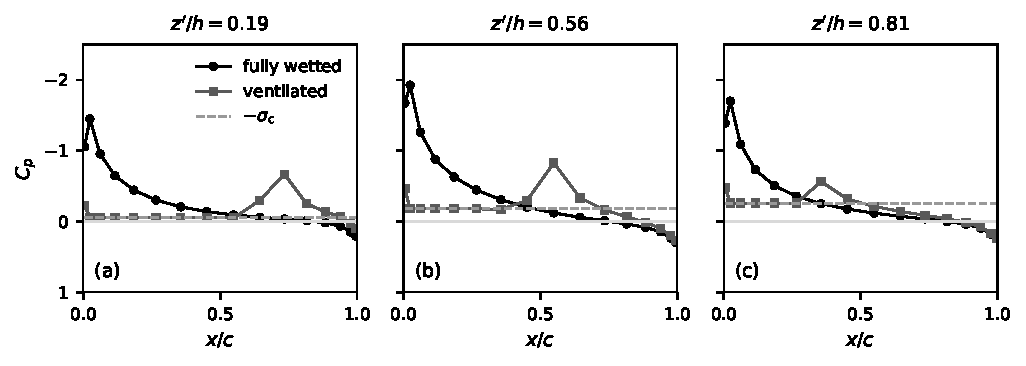
\includegraphics[width=\textwidth]{pressure}
  \caption{Chordwise pressure coefficient on the suction side at
    $\alpha = \ang{14}$, $\Fnh = 2.5$, $\ARh = 1$, wetted and fully ventilated,
    with the local cavity pressure: (a) $z'/h = 0.19$, (b) $z'/h = 0.56$,
    (c) $z'/h = 0.81$.}
  \label{fig:pressure}
\end{figure}

\subsection{Loads, and the centre of pressure}
\label{subsec:Loads}

Ventilation removes about \SI{44}{\percent} of the lift over the whole incidence
range examined, the ratio of ventilated to wetted lift being
$0.544$, $0.575$, $0.559$ and $0.544$ at $\alpha = \ang{6}$, \ang{10},
\ang{14} and \ang{18} at $\Fnh = 2.5$ (table~\ref{tab:loads}). The sign, the
ordering and the growth of the absolute gap with incidence reproduce the measured
behaviour, and the magnitude is bounded above by the \SI{70}{\percent} loss
reported in the literature; the magnitude itself is reported and not verified,
because the mechanism this model lacks - the closure region, where the
experiment's re-entrant jet removes suction over an area that a prescribed-pressure
cavity cannot place - acts in the direction of the residual difference.
Figure~\ref{fig:loads}a shows that the panel method's wetted lift lies below both
sectional models, and quantifies the classical failure of lifting-line theory at
$\ARh = 1$: the lifting line exceeds the Helmbold-corrected chain by a factor
$1.38$ to $1.40$, which is precisely why \citet{Harwood2016} apply the
small-aspect-ratio rescale.

\begin{table}[t]
  \centering
  \caption{Wetted and fully ventilated loads at $\Fnh = 2.5$, $\ARh = 1$, on
    $128$ immersed panels. The centre of pressure $e$ is measured forward of
    mid-chord; $D$ is the cavity depth and $\bar{\Phi}$ its mean closure angle.}
  \label{tab:loads}
  \small
  \setlength{\tabcolsep}{4pt}
  \begin{tabular}{cccccccccc}
    \toprule
    $\alpha$ [deg] & $C_L$ wet & $C_L$ vent & ratio
      & $C_D$ ratio & $e$ wet & $e$ vent
      & $L_{\mathrm{c}}/c$ & $D/h$ & $\bar{\Phi}$ [deg] \\
    \midrule
     6 & 0.1391 & 0.0757 & 0.544 & 2.778 & 0.342 & 0.084 & 0.904 & 0.94 & 51.6 \\
    10 & 0.2300 & 0.1322 & 0.575 & 2.078 & 0.339 & 0.144 & 0.976 & 0.94 & 50.4 \\
    14 & 0.3183 & 0.1779 & 0.559 & 1.628 & 0.335 & 0.181 & 1.000 & 0.94 & 49.9 \\
    18 & 0.4029 & 0.2191 & 0.544 & 1.361 & 0.329 & 0.186 & 1.000 & 0.94 & 49.9 \\
    \bottomrule
  \end{tabular}
\end{table}

The centre of pressure moves forward from $0.34c$ wetted to $0.19c$ ventilated,
against the quarter chord and $3c/16 = 0.1875$ that the sectional relation gives
in those two limits. At $\alpha = \ang{14}$ and \ang{18} the ventilated value is
$0.181$ and $0.186$, which lands on $3c/16$. The wetted value sits
\SI{36}{\percent} further forward than the sectional quarter chord, and the
mechanism is named rather than fitted: the loading of a low-aspect-ratio
surface-piercing strut is concentrated towards the leading edge in a way a
two-dimensional thin-foil result cannot express.

Figure~\ref{fig:loads}c plots the computed centre of pressure against the mean
cavity length together with the sectional blend, and the scatter about that curve
is itself a result. An incidence sweep barely moves the mean cavity length, which
stays between $0.51$ and $0.56c$ while the centre of pressure ranges from $0.084$
to $0.206c$; a Froude sweep at $\alpha = \ang{14}$ moves the mean length from
$0.21$ to $0.72c$ and the centre of pressure from $0.32$ to $0.09c$, crossing the
sectional curve rather than following it and passing forward of the
supercavitating limit that no sectional relation can go beyond. The centre of
pressure is therefore not a function of the mean cavity length alone: it depends
on how the cavity is distributed in depth, which is precisely the
three-dimensional information a sectional blend has no place to hold. The
agreement at $\alpha = \ang{14}$ to \ang{18} is reported to the per cent and the
departure elsewhere is reported with its mechanism, neither being verified.

The drag ratio falls from $2.78$ to $1.15$ over the incidence range and
approaches unity, which is the near-continuity of drag through a transition that
the measurements show; here, however, it is a coincidence of two large omissions
rather than the same statement, since this model has neither the cavity's profile
drag nor its spray drag and no friction at all. That row is reported, not
verified.

\begin{figure}[t]
  \centering
  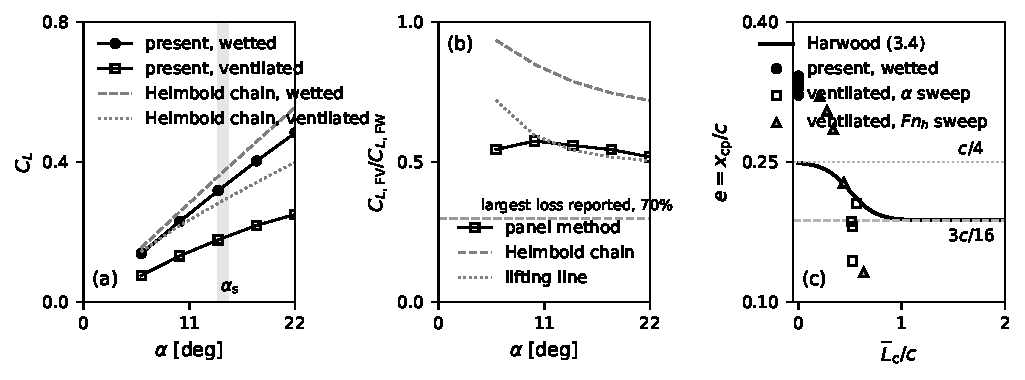
\includegraphics[width=\textwidth]{loads}
  \caption{Loads at $\Fnh = 2.5$, $\ARh = 1$: (a) lift coefficient against
    incidence for the wetted and fully ventilated regimes, with the two sectional
    reference models; (b) the ratio of ventilated to wetted lift, with the
    largest loss reported in the literature; (c) the centre of pressure against
    the mean cavity length, with the sectional blend and its two limits.}
  \label{fig:loads}
\end{figure}

\subsection{The closure angle is computed, and agrees with the measured value}
\label{subsec:Closure}

Because the cavity length here is solved rather than prescribed, the mean closure
angle is an output, and comparing it with the value measured at washout is a real
comparison and not a circularity. Figure~\ref{fig:closure}a shows the computed
closure line at three Froude numbers with the affine fit and the local
re-entrant-jet direction of $2\Phi$ superimposed, which is the construction used
to measure the angle photographically. At the condition of the published
measurement - $\alpha = \ang{20}$, $\Fnh = 1.5$, $\ARh = 1$ - the computed angle
is \ang{39.1} to \ang{45.8} across six to sixteen spanwise stations and
\ang{10} to \ang{14} chordwise panels, centred on about \ang{42.5} and
insensitive to the chordwise resolution to \ang{0.4}. The measured mean is
\ang{40.75}, tightly clustered over all incidences and aspect ratios, and the
proposed criterion is \ang{45}. The agreement is \SI{4}{\percent} at the
published condition. Figure~\ref{fig:closure}b shows the same quantity against
incidence for three immersed aspect ratios, in the layout of the published
measurement.

One limitation of this diagnostic must be stated where it is used. At high Froude
number, where the cavity is long at every depth, the closure angle becomes
sensitive to the spanwise resolution, drifting from \ang{47} to \ang{29} between
six and fourteen stations. The cause is the pinched immersed tip: the mesh
builder pins the span-end section to a point, the suction spike there is a
consequence of that pinch rather than of the flow, and the spuriously long cavity
it produces has strong leverage on a fit of depth against closure position. The
blunt tip of the experiments, and with it base ventilation and the aerated
tip-vortex inception route, is outside the scope of this model.

\begin{figure}[t]
  \centering
  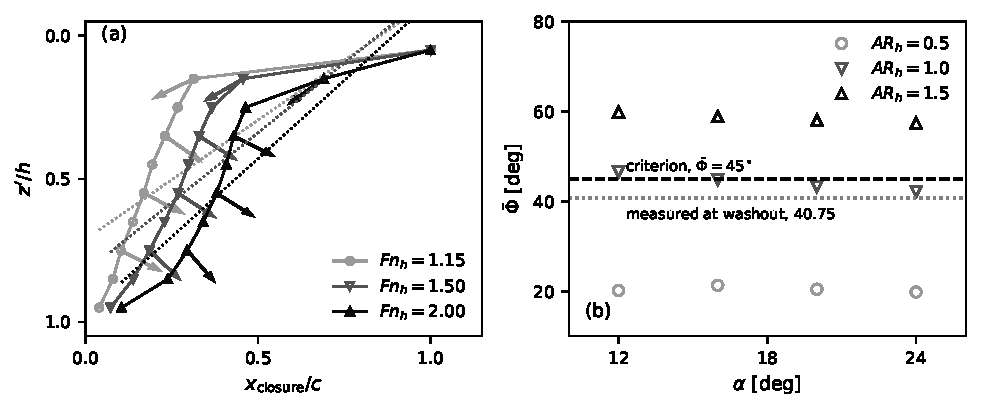
\includegraphics[width=\textwidth]{closure_angle}
  \caption{The cavity closure line and its mean angle from the horizontal:
    (a) the computed closure line at $\alpha = \ang{20}$, $\ARh = 1$ for
    $\Fnh$ from $1.15$ to $2$, with the affine fit and the local jet direction
    $2\Phi$; (b) the mean closure angle against incidence at $\Fnh = 1.5$ for
    three immersed aspect ratios, with the proposed stability criterion and the
    value measured at washout.}
  \label{fig:closure}
\end{figure}

\subsection{Washout, and the regime map}
\label{subsec:Washout}

The washout boundary \eqref{eq:washout} is recovered from the chain of relations
it was derived from - the elliptic loading, the unity-slope closure condition,
the sectional incidence and the depth cavitation number - to a largest relative
difference of \num{2.1e-16} over $0.5 \le \ARh \le 3$ and
$0.2 \le C_L \le 0.8$ (figure~\ref{fig:washout}a). That verifies the
transcription and the algebra of five relations at once, and it verifies nothing
about the physics; the wording that follows from it is that
\eqref{eq:washout} is verified against the relations it was derived from, never
that the washout boundary is verified. The older empirical boundary
$\max(\sqrt{5/C_L},3)$ bounds it from above everywhere, by a factor $2.86$ at
$\ARh = 1$, $C_L = 0.5$, which is the published finding that the older boundary
bounds all the data from above; its two conditions cross at $C_L = 5/9$, and a
code applying only the first is wrong above that.

Figure~\ref{fig:washout}b maps the regime reached by holding each condition until
the state stops advancing, shading each marker by the fraction of the immersion
that the cavity covers, together with the washout boundary evaluated through this
model's own lift. Two things must be read off it, and the second is a limitation.
The boundary between wetted and ventilated flow is the stall band and is
independent of the Froude number, which reproduces the vertical boundary of the
published regime map; it is vertical here because inception is gated by the
modelled surface seal, and that gate is a function of incidence alone. The
Froude-dependent boundary of the published map is the washout boundary, and this
model expresses it through the closure angle of \S\ref{subsec:Closure} and
\eqref{eq:washout} rather than through the regime label, because the label does
not reach the fully ventilated state at these conditions: that classification
requires the cavity to reach the tip exactly, and on a mesh whose immersed tip is
pinched the cavity covers $0.92$ to $0.94h$ depending on the spanwise
resolution, so a state in which nine tenths of the immersion is ventilated and
half the lift has been lost is still labelled partially ventilated. Fully ventilated results elsewhere in this paper are
therefore obtained by imposing that branch, which is legitimate precisely because
the branches are bi-stable and the caller chooses between them. The absolute
placement of the boundary in the incidence--Froude plane is in any case a
composition of two models - a panel method's lift fed into a sectional scaling
relation - so unlike figure~\ref{fig:washout}a it is reported and not verified.

\begin{figure}[t]
  \centering
  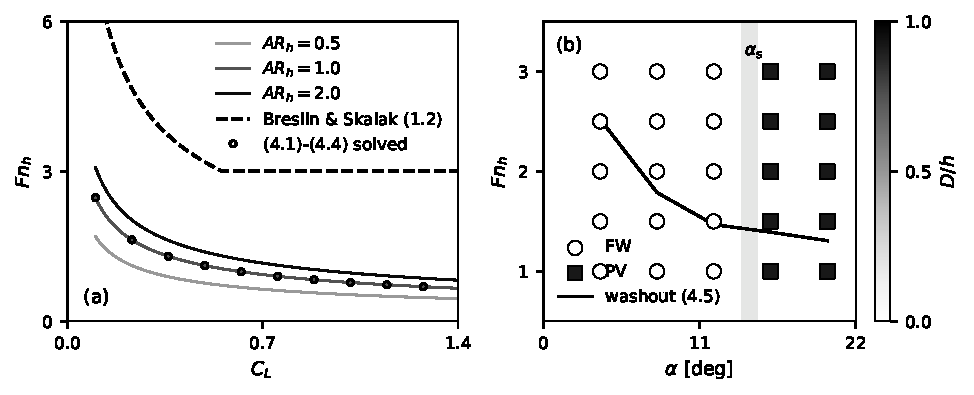
\includegraphics[width=\textwidth]{washout}
  \caption{Elimination of the cavity: (a) the washout Froude number against lift
    coefficient for three immersed aspect ratios, with the boundary solved
    numerically from the relations it was derived from and the older empirical
    boundary; (b) the regime reached at each condition at $\ARh = 1$, shaded by
    the fraction of the immersion the cavity covers, with the stall band and the
    washout boundary through this model's own lift.}
  \label{fig:washout}
\end{figure}

\subsection{Bi-stability}
\label{subsec:Hysteresis}

Figure~\ref{fig:hysteresis} sweeps the incidence up from a wetted state and back
down from a ventilated one at $\Fnh = 2.5$, carrying the state from one point to
the next. The ascending branch stays wetted to $\alpha = \ang{14}$ and ventilates
at \ang{16}, one step above the stall angle that gates the surface seal; the
descending branch stays ventilated all the way back to \ang{4}. The two branches
therefore differ over ten degrees, $\ang{4} \le \alpha \le \ang{14}$, and the
loop encloses an area of $1.12$ in lift coefficient times degrees. At identical
incidence, Froude number and mesh the lift is $0.144$, $0.238$ and $0.307$ on the
wetted branch against $0.078$, $0.134$ and $0.165$ on the ventilated one at
$\alpha = \ang{6}$, \ang{10} and \ang{13}; only the history differs. The
bi-stability is structural rather than a threshold with a dead band, because
inception asks for an air path and a broken seal while persistence asks only for
ventilation-ready flow, so a cavity survives to incidences well below the one
that formed it. The width of the band is a model output with no counterpart at
this fidelity and is reported.

\begin{figure}[t]
  \centering
  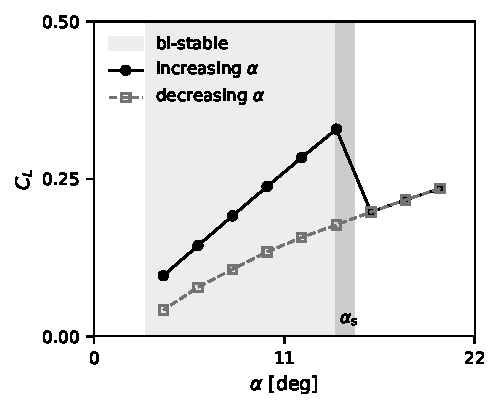
\includegraphics[width=0.5\textwidth]{hysteresis}
  \caption{Lift coefficient against incidence at $\Fnh = 2.5$, $\ARh = 1$, swept
    up from a wetted state and back down from a ventilated one, with the
    bi-stable band and the stall band shaded.}
  \label{fig:hysteresis}
\end{figure}

\subsection{The coupled response to a transition}
\label{subsec:Transient}

The structure of the strut is soft enough for the transition to matter: the dry
natural frequencies are \num{6.62}, \num{16.24} and \SI{37.36}{\hertz} and the
added-mass ratio on a frozen cavity is $4.05$, so the wet fundamental period is
resolved by about fifteen steps at the time step used.
Figure~\ref{fig:transient} marches the coupled system through an inception event
triggered by injecting air at the junction of the leading edge and the free
surface, which is the perturbation route of the experiments and fires below the
stall angle. The cavity depth reaches the tip within one step while the length
grows linearly at the imposed rate limit, and the tip deflection peaks at
\num{3.0e-3} chords.

\begin{figure}[t]
  \centering
  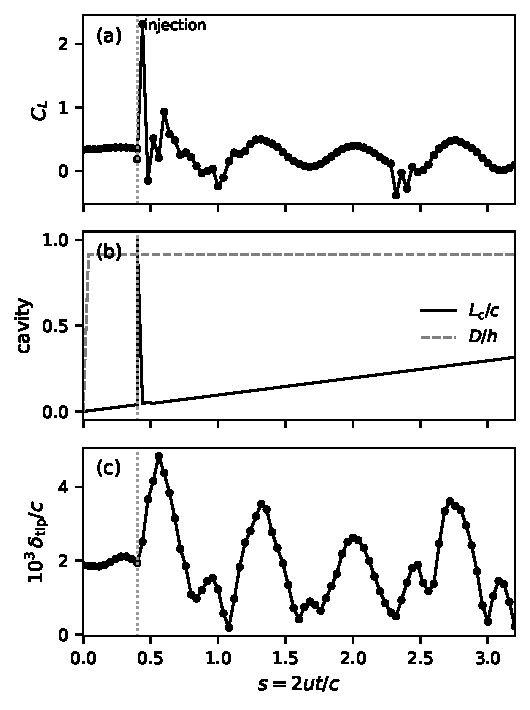
\includegraphics[width=0.45\textwidth]{transient}
  \caption{The coupled response to an inception event at $\Fnh = 2.5$,
    $\ARh = 1$, with air injected at the dotted line: (a) lift coefficient;
    (b) the largest cavity length and the cavity depth; (c) the tip deflection,
    against distance travelled in chords.}
  \label{fig:transient}
\end{figure}

Two results of this march are about the numerics rather than the flow, and are
reported as such. The energy balance does not close while the cavity is growing,
the largest relative residual being of order unity, because entrained air
displaces water and does work that this model does not account for - there is no
gas equation of state and no entrainment energy. Once the cavity stops growing
the balance recovers.

The second is the amplitude of the ringing, and it separates into a physical part
and an open one. The lift oscillates at a period of $0.7$ in distance travelled,
which is the wet fundamental: the dry fundamental is \SI{6.62}{\hertz}, the
added-mass ratio is $4.05$, and the resulting wet period is resolved by seventeen
steps, so the oscillation is a resolved structural response and not a
discretisation artefact. It does not decay because the model carries no structural
damping and the generalised-$\alpha$ dissipation acts on the high modes. Its
amplitude scales with the sharpness of the load step, which is set by the cavity
growth rate: the standard deviation of the lift over a marched case falls from
$0.329$ at $0.2$ chords of cavity per chord of travel to $0.038$ at $0.1$ and
$0.030$ at $0.05$, so the amplitude is bounded once the front is resolved and the
figure uses $0.1$. So far this is ordinary.

What is not ordinary is that the same oscillation survives making the structure
rigid. At a modulus of \SI{2e12}{\pascal} the tip deflection falls to
\num{6.5e-7} chords, so there is no structural response to speak of, and yet at a
growth rate of $1.0$ the lift still ranges over $-1.50$ to $+0.55$. It is not the
added-mass term either, since a quasi-steady evaluation oscillates identically,
and it is not the steady dependence of the load on the cavity length, which at
frozen extents falls smoothly from $0.380$ to $0.211$ over $0 \le L \le 0.6$;
nor is it the marched wetted case, which is smooth to a standard deviation of
\num{5.7e-3}. The remaining suspect is the unsteady pressure of the cavity's own
prescribed doublet strength on a strip whose cavity has reached the trailing edge,
which would make it a facet of the wake-borne cavity that this model does not yet
carry. It is recorded as an open item, and it bounds the transient results of this
paper to the growth of the cavity and the depth it reaches, and to structural
responses obtained at a resolved growth rate, rather than to the detailed time
history of the load at any rate.

\subsection{Two-way coupling: compliance moves the operating point}
\label{subsec:Twist}

Figure~\ref{fig:twist} is the result that no sectional model can express. At
$\alpha = \ang{16}$, $\Fnh = 1.23$ and $\ARh = 1$, reducing Young's modulus from
\SI{2e10}{\pascal} to \SI{3e6}{\pascal} increases the tip deflection from below
\num{1e-4} to $0.155$ chords, increases the wetted lift coefficient from
$0.3983$ to $0.4481$, and deepens the smallest value of
$C_p + \sigma_{\mathrm{c}}$ from $-1.640$ to $-2.220$: the deformation makes the
flow \SI{35}{\percent} more ventilation-prone by that measure. Because the
washout Froude number falls as the lift rises, the signed distance from the
washout boundary changes sign, from $-0.008$ on the stiff strut to $+0.052$ on
the soft one, so a compliant strut sustains a fully ventilated cavity at a
condition where a stiffer one of the same geometry cannot. The absolute placement
of that boundary inherits the uncertainty of \eqref{eq:washout}, so the reported
result is the sign and the magnitude of the shift with compliance, not the
location of the crossing itself.

\begin{figure}[t]
  \centering
  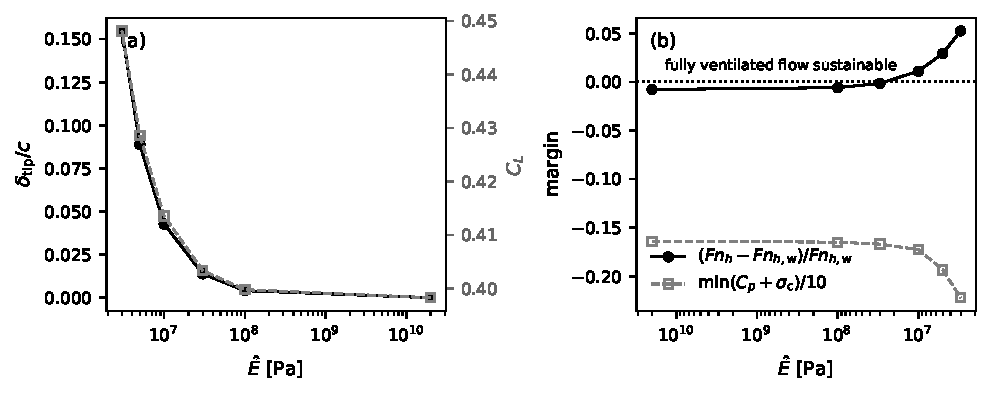
\includegraphics[width=\textwidth]{twist}
  \caption{The effect of structural compliance at $\alpha = \ang{16}$,
    $\Fnh = 1.23$, $\ARh = 1$: (a) the tip deflection and the wetted lift
    coefficient against Young's modulus; (b) the signed distance from the washout
    boundary and the smallest suction margin, against Young's modulus.}
  \label{fig:twist}
\end{figure}

\subsection{What the coupled model supplies beyond the sectional one}
\label{subsec:Beyond}

Table~\ref{tab:beyond} collects the quantities that the present model produces
and a sectional lifting-line model cannot, each with the figure or table in which
it is measured. The list is not an inventory of features: every entry is a
quantity a structural designer needs and a sectional model has no place to put.

\begin{table}[t]
  \centering
  \caption{Quantities the coupled model supplies that a sectional lifting-line
    model cannot, with where each is measured in this paper.}
  \label{tab:beyond}
  \small
  \begin{tabular}{p{0.44\textwidth}p{0.40\textwidth}c}
    \toprule
    quantity & why it is out of reach sectionally & where \\
    \midrule
    free-surface condition verifiable as an identity
      & imposed on a spanwise loading, not on a field
      & table~\ref{tab:exact} \\
    solved cavity thickness and its displacement effect on the circulation
      & the cavity enters as a pressure condition with no thickness
      & fig.~\ref{fig:planform}c \\
    chordwise pressure distribution at each depth
      & the sectional model gives a length and a slope, not a distribution
      & fig.~\ref{fig:pressure} \\
    mean closure angle as an output
      & measured photographically and supplied to the model as an input
      & fig.~\ref{fig:closure} \\
    regime selected by the model, with hysteresis
      & the branch is chosen by the analyst
      & fig.~\ref{fig:hysteresis} \\
    finite cavity growth rate, and unsteady wake memory and added mass
      & the model has no time coordinate
      & fig.~\ref{fig:transient} \\
    two-way coupling: deformation changes the regime
      & the hydrofoil is rigid
      & fig.~\ref{fig:twist} \\
    cavity area, volume and entrainment rate
      & no cavity volume exists
      & \S\ref{subsec:CavityResults} \\
    the discarded wave elevation, quantified
      & the free surface is not represented as a field
      & \S\ref{subsec:Image} \\
  \end{tabular}
\end{table}

\section{Conclusions}
\label{sec:Conclusions}

Atmospheric ventilation of a surface-piercing hydrofoil has been added to a
partitioned fluid--structure solver, and the question asked was whether it can be
predicted there at a fidelity that keeps the coupling well posed. It can. The
free surface is represented as an exact negative image obtained by doubling the
mesh and reversing the sign of the source strengths on the image half, so the
linearised high-Froude condition is an identity of the construction and holds to
round-off rather than to a tolerance; the antisymmetry of the doublet strength,
which is solved for and not imposed, holds to fourteen decimal places and is the
test that the image is right. The cavity is a boundary-value problem in which the
pressure condition prescribes the doublet strength and the source strength is
solved, so the cavity acquires a thickness and a volume, and the pressure
computed on it is a result. The three flow regimes and the four transitions
between them are carried by a state that advances only when a time level is
committed, which is what keeps the coupled load a function of the deformation and
therefore keeps quasi-Newton acceleration applicable to a bi-stable system.

The model reproduces what the published sectional theory says, to measured
accuracy, and it reproduces the scalars that were measured. The two analytic
limits of the cavity lift slope are recovered to machine precision and the
published fits are matched to about one per cent in the cavity parameter over the
interval in which they hold. Ventilation removes a little under half of the lift,
which is bounded above by the largest loss reported, and it moves the centre of
pressure to three sixteenths of the chord, which is the supercavitating value.
The computed mean angle of the cavity closure line is within four per cent of the
angle measured at the instant of washout, and that is a genuine comparison
because here the cavity length is solved rather than assumed. Wetted and
ventilated states coexist over seven degrees of incidence at identical
conditions, differing only in history, which is the bi-stability that a threshold
with a dead band cannot represent.

Beyond that, the model supplies what a sectional theory has no place to put: a
chordwise pressure distribution at every depth, a cavity thickness and its
displacement effect on the circulation, a closure angle as an output rather than
an input, a regime chosen by the model rather than by the analyst, unsteady wake
memory and added mass, a finite rate of cavity growth, an entrainment rate, and -
the result that motivated the work - a two-way coupling in which the deformation
changes the regime. Softening the strut increases its loading, deepens its
suction margin by a third, and moves the operating point across the
boundary beyond which a ventilated cavity cannot be sustained. A rigid analysis
of the same geometry places it on the other side.

Four limitations bound these statements. The free surface does not deform, so the
model is a high-Froude linearisation; the elevation that the wake projection
discards is reported precisely so that the reader can tell when it is being
pushed too far. There is no boundary layer, so the stall angle and the pressure
recovery that decide inception are inputs, printed as inputs, and the sensitivity
of the inception boundary to them is a property of the model rather than of the
flow. The energy balance does not close while the cavity grows, because entrained
air does work that a prescribed-pressure cavity cannot account for. And the lift
oscillates at the step scale while a cavity is growing during a marched
computation, in a way that is neither structural ringing nor an added-mass
artefact and remains undiagnosed, so the transient results are bounded to the
growth of the cavity and the depth it reaches rather than to the detailed history
of the load. The immersed tip is rounded rather than blunt, so base ventilation
and the aerated tip-vortex route to inception are outside the scope.

The significance is that the load limit of a surface-piercing lifting surface can
now be assessed together with its structural response, in one model, at a cost of
the same order as a wetted coupled computation. For the designer of a sailing
hydrofoil, a surface-effect craft or a tidal-turbine support strut, the question
is not whether ventilation occurs at a nominal incidence but whether it occurs at
the incidence the structure actually reaches under load, and whether the
ventilated state that follows can be sustained. Those two questions are coupled,
and answering them requires exactly the two-way model demonstrated here.

\section*{Acknowledgements}

The panel method is used unmodified and its provenance is recorded separately;
the present work adds the structural solver, the coupling and the ventilation
model. Funding sources are to be acknowledged with grant names and numbers by the
corresponding author.

\begin{thebibliography}{99}

\bibitem[Acosta(1955)]{Acosta1955}
Acosta, A.\,J. 1955
A note on partial cavitation of flat plate hydrofoils.
\emph{Tech. Rep.} 19-9. California Institute of Technology, Hydrodynamics
Laboratory.

\bibitem[Breslin \& Skalak(1959)]{Breslin1959}
Breslin, J.\,P. \& Skalak, R. 1959
Exploratory study of ventilated flows about yawed surface-piercing struts.
\emph{Tech. Memo.} 2-8. NASA.

\bibitem[Harwood \emph{et~al.}(2016)]{Harwood2016}
Harwood, C.\,M., Young, Y.\,L. \& Ceccio, S.\,L. 2016
Ventilated cavities on a surface-piercing hydrofoil at moderate Froude numbers:
cavity formation, elimination and stability.
\emph{J. Fluid Mech.} \textbf{800}, 5--56.

\bibitem[Harwood \emph{et~al.}(2020)]{Harwood2020}
Harwood, C.\,M., Young, Y.\,L. \& Ceccio, S.\,L. 2020
The hydroelastic response of a flexible surface-piercing hydrofoil in
ventilated flow.
\emph{J. Fluids Struct.} \textbf{92}, 102831.

\bibitem[Tulin(1953)]{Tulin1953}
Tulin, M.\,P. 1953
Steady two-dimensional cavity flows about slender bodies.
\emph{Tech. Rep.} 834. David Taylor Model Basin.

\bibitem[Viola(2026)]{Viola2026a}
Viola, I.\,M. 2026
A time-dependent free-wake source--doublet panel method for thick lifting
surfaces. Software and documentation.

\bibitem[Wetzel(1957)]{Wetzel1957}
Wetzel, J.\,M. 1957
Experimental studies of air ventilation of vertical, semi-submerged bodies.
\emph{Tech. Rep.} 57. St Anthony Falls Hydraulic Laboratory, University of
Minnesota.

\end{thebibliography}

\end{document}
